\section[]{پرسش ۱.}
می‌دانیم پس از آن‌که یک مدل یادگیرنده مرحله آموزش خود را سپری کرد، باید توسط چندین معیار، ارزیابی و سنجیده شود. همچنین اگر مسئله موردنظر از نوع رگرسیون باشد، خروجی مدل یک بردار مانند $\hat{Y}$ و مقادیر برچسب نیز درون بردار دیگری مانند $Y$ قرار دارند که همگی از نوع اعداد پیوسته هستند. 

\begin{equation*}
	Y = \begin{bmatrix} y_{0} \\ y_{1} \\ \vdots \\ y_{n} \end{bmatrix},\:\:\:\:\:\: \hat{Y} = \begin{bmatrix} \hat{y}_{0} \\ \hat{y}_{1} \\ \vdots \\ \hat{y}_{n} \end{bmatrix}
\end{equation*}
به عنوان مثال یکی از معیارهای ارزیابی مدل‌های رگرسیونی، میانگین مربع خطا
\LTRfootnote{Mean Square Error}
می‌باشد که به صورت زیر بیان می‌شود:
\begin{equation}
	\label{eq1}
	MSE = \frac{1}{N} \sum_{i=1}^{N} (\hat{y_i} - y_i)^2
\end{equation}

\subsection*{الف.}
مجموعه داده‌ای از مساحت خانه و قیمت آن به همراه پیش‌بینی مدل به شما داده شده است (جدول \ref{tb1}). در شکل \ref{fig1} نقاط این مجموعه داده با درنظر گرفتن مساحت خانه در محور $x$ و قیمت آن در محور $y$ به همراه فرضیه $h$ که یک خط تخمین زده شده توسط الگوریتم رگرسیون خطی است، نشان داده شده است. باتوجه به خط فرضیه تخمین زده شده، هر نقطه از این مجموعه داده که به خط فرضیه داده شود، دارای خطای $e_i$ است. مقدار $MSE$ را برای این مجموعه داده محاسبه کرده و مقدار حاصل از آن را توصیف کنید و توضیح دهید که این معیار ارزیابی چه معایب و مزایایی دارد. (می‌توانید با ارائه یک مثال، توضیحات کامل‌تری ارائه دهید)
\\
\\ \\ \\ \\ \\ \\ 

\subsection*{ب.}
دو معیار ارزیابی دیگر برای مسائل رگرسیون انتخاب کرده و مقدار آن‌ها را برای مجموعه داده جدول \ref{tb1} محاسبه کنید. همچنین توضیح دهید که هرکدام از چه رابطه‌ای بدست می‌آیند و معایب و مزایای آن‌ها نسبت به یکدیگر چگونه است.

\begin{figure}
	\centering
	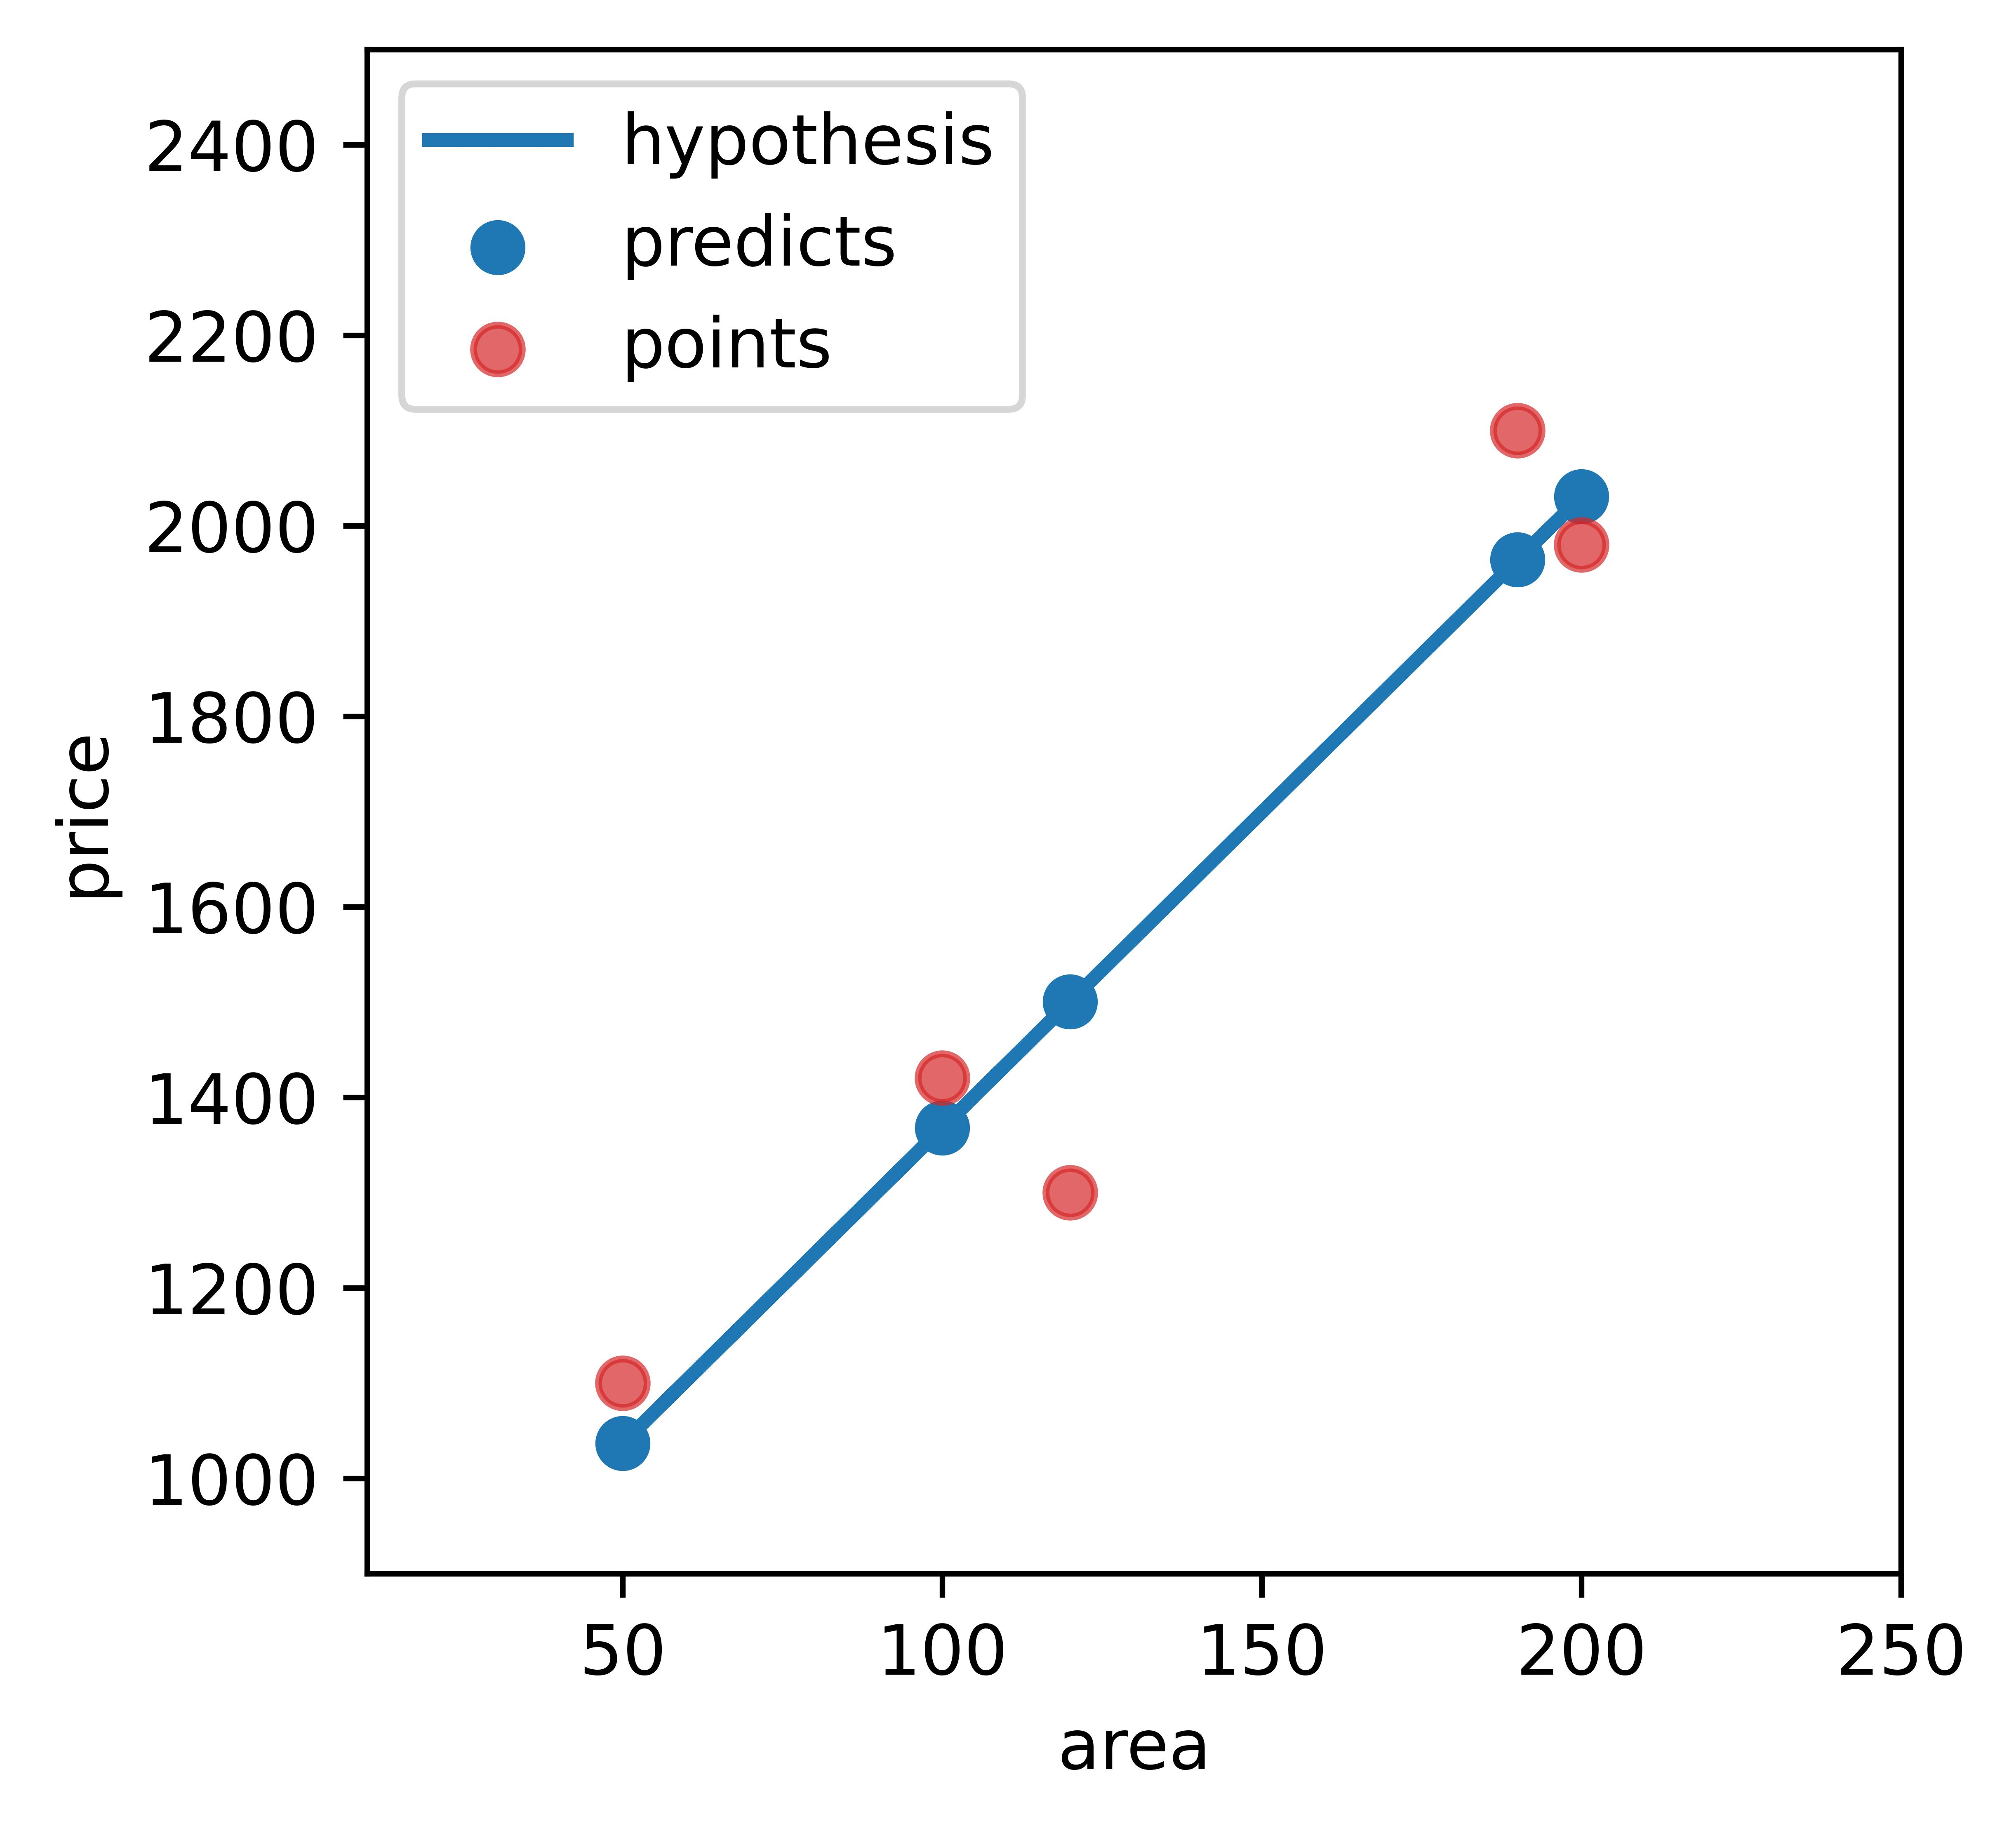
\includegraphics[width=5cm, height=4.5cm]{figure_01}
	\caption{
		نمایش دو بُعدی داده‌ها به همراه فرضیه تخمین زده شده. برای اطلاعات بیشتر و کد زدن با این مجموعه داده، می‌توانید از کدی که در 
		\href{https://github.com/Sinahjafari/machine-learning-course/blob/main/jupyter_notebooks/regression/simple_regression_for_evaluation.ipynb}{
		\big] این \big[
		}
		آدرس نوشته شده است استفاده کنید.
	}
	\label{fig1}
\end{figure}

\begin{table}
	\centering
	\caption{مجموعه داده قیمت خانه‌ها}
	\label{tb1}
	\begin{tabular}{ccc}
		\toprule
		قیمت پیش‌بینی شده & قیمت واقعی & مساحت خانه \\
		\midrule
		1964 & 2100 & 190 \\
		2031 & 1980 & 200 \\
		1368 & 1420 & 100 \\
		1037 & 1100 & 50 \\
		1500 & 1300 & 120 \\
		\bottomrule
	\end{tabular}
\end{table}